%%%%%%%%%%%%%%%%%%%%%%%%%%%%%%%%%%%%%%%%%%%%%%%%%%%%%%%%%%%%%%%%%%%
%TO AVOID FORMATTING ISSUES, COMPILE THIS ONLY AT WWW.OVERLEAF.COM%
%%%%%%%%%%%%%%%%%%%%%%%%%%%%%%%%%%%%%%%%%%%%%%%%%%%%%%%%%%%%%%%%%%%
%AUTHOR: ABHINAV BAKSHI
%CLASS:  BE C 302
%%%%%%%%%%%%%%%%%%%%%%%%%%%%%%%%%%%%%%%%%%%%%%%%%%%%%%%%%%%%%%%%%%%
\documentclass[a4paper,12pt]{article}
\usepackage{graphicx}
%To use this font, you need XeTex or LuaTex, prefer openleaf
\newenvironment{codefont}{\fontfamily{ccr}\selectfont}{\par}

\title{
	\normalfont \normalsize 
	\textsc{Pimpri Chinchwad College of Engineering \\ 
		Computer Laboratory - IV} \\
	[10pt] 
	\rule{\linewidth}{0.5pt} \\[6pt] 
	\huge Assignment No - B6 \\
	\rule{\linewidth}{2pt}  \\[10pt]
}
\author{}
\date{\normalsize}


\begin{document}
\maketitle

%%%%%%%%%%%%%%%%%%%%%%%
% FOR A NUMBERED LIST
% \begin{enumerate}
% \item Your_Item
% \end{enumerate}
%%%%%%%%%%%%%%%%%%%%%%%
% FOR A BULLETED LIST
% \begin{itemize}
% \item Your_Item
% \end{itemize}
%%%%%%%%%%%%%%%%%%%%%%%
% TO IMPORT AN IMAGE
% \includegraphics[width=\textwidth]{name_of_file}
% \textwidth makes the picture the width of the paragraphs
%%%%%%%%%%%%%%%%%%%%%%%%%%%%%%
% TO CREATE A FIGURE WITH A NUMBER AND CAPTION
% \begin{figure}
% \includegraphics[width=\textwidth]{image}
% \caption{Your Caption Goes Here}
% \label{your_label}
% \end{figure}
% REFER TO YOUR FIGURE LATER WITH
% \ref{your_label}
% LABELS NEED TO BE ONE WORD
%%%%%%%%%%%%%%%%%%%%%%%%%%%%%
% TO ADD CODE
% \begin{codefont}
% Some code in "courier" font
%\end{codefont}
%%%%%%%%%%%%%%%%%%%%%%%%%%%%%
\section{Aim}
	\paragraph{} Implement OBST Tree search using HPC task sub-division. Merge the results to get final result.
	
\section{Objective}
	\begin{itemize}
		\item To understand concept of OBST.  
		\item To effectively use multi-core or distributed, concurrent/Parallel environments.  
		\item To develop problem solving abilities using Mathematical Modeling.  
		\item To develop time and space efficient algorithms.  
	\end{itemize}
	
\section{Software Requirements}
	\begin{itemize}
		\item Linux or Windows Operating System
		\item Python
	\end{itemize}
	
\section{Mathematical Model}
	Let S be the system, 	 													\\
	S : (s, e, I, O, Fm, Ft, St) 												\\\\
	Where, 	\\
	 s: Start State , i.e. taking input e: End State i.e. search result I: Set of inputs 	 														\\
	I: size of array, array elements O: 										\\
	Set of outputs 	 															\\
	O: Sorted array, position of element 										\\
	Fm: Main function or algorithm that gives specific Output i.e. main() 	 	\\
	Ft: Failure State. i.e. Getting Exceptions as Output after inserting characters, string or float values as Input. 	 							\\
	St : Success State. i.e. Getting the Expected Element and its position in array as output. 															\\
	
	
\section{Theory}
	\subsection{OSBT:} An optimal binary search tree is a binary search tree for which the nodes are arranged on levels such that the tree cost is minimum. For the purpose of a better presentation of optimal binary search trees, we will consider “extended binary search trees”, which have the keys stored at their internal nodes. Suppose “n” keys k1, k2, … , k n are stored at the internal nodes of a binary search tree. It is assumed that the keys are given in sorted order, so that k1< k2 < … < kn. An extended binary search tree is obtained from the binary search tree by adding successor nodes to each of its terminal nodes as indicated in the following figure by squares. 
	
	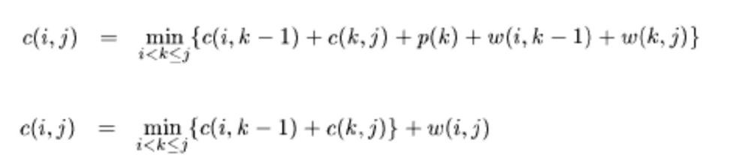
\includegraphics[width=\textwidth]{obst_m1}
	
	\vspace{50px}
	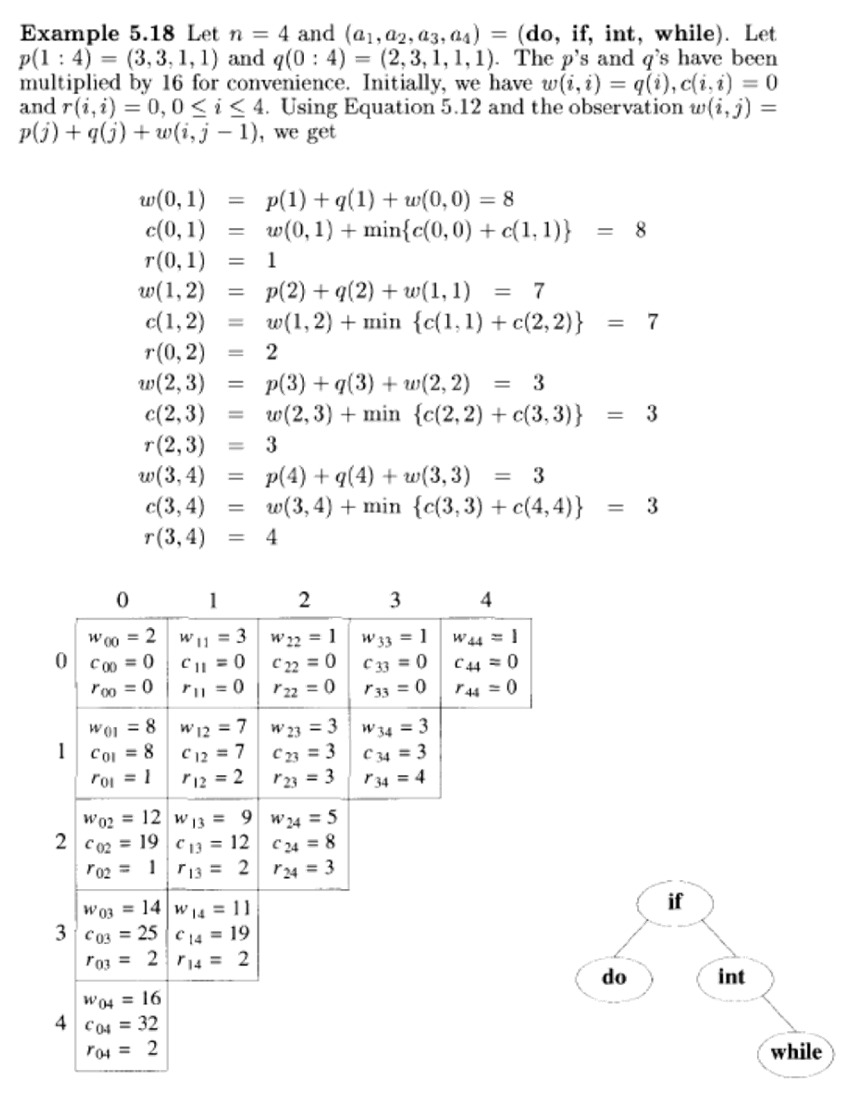
\includegraphics[width=\textwidth]{obst_m2}
	\newpage
	
	\subsection{Advantage:}
	The major advantage of binary search trees over other data structures is that the related sorting algorithms and search algorithms such as in-order traversal can be very efficient, they are also easy to code. 
	\vspace{30px}
	
	\subsection{Disadvantage:}
	\begin{itemize}
		\item The shape of the binary search tree totally depends on the order of insertions and deletions, and can become degenerate.  
		
		\item When inserting or searching for an element in a binary search tree, the key of each visited node has to be compared with the key of the element to be inserted or found.  
		
		\item The keys in the binary search tree may be long and the run time may increase.  
		
		\item After a long intermixed sequence of random insertion and deletion, the expected height of  	the tree approaches square root of the number of keys, √N, which grows much faster  than log N.  
		
	\end{itemize}
	
	\subsection{Analysis:}
	The optimal binary search tree has a time complexity of O(n\^3). It’s space efficiency is only O(n\^2). It can possibly be lowered to complexity O(n\^2) with smarter recursive functions and smaller ranges of values. 

		
\section{Algorithm}
	\paragraph{} Suppose “n” keys k1, k2, … , k n are stored at the internal nodes of a binary search tree. It is assumed that the keys are given in sorted order, so that k1< k2 < … < kn. An extended binary search tree is obtained from the binary search tree by adding successor nodes to each of its terminal nodes as indicated in the following figure by squares. 
	
	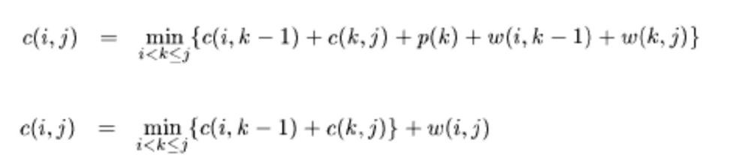
\includegraphics[width=\textwidth]{obst_m1}


\section{Testing}
\subsection{Positive Testing}
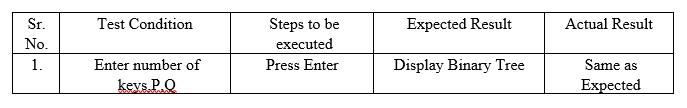
\includegraphics[width=\textwidth]{obst_positive}

\subsection{Negative Testing}
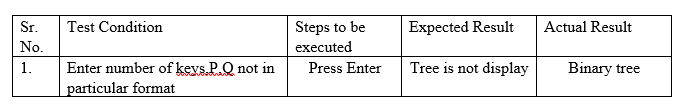
\includegraphics[width=\textwidth]{obst_negative}

\vspace{50px}


\section{Conclusion}
From this assignment we have studied concept of OBST and developed time and space efficient algorithm using multicore , concurrent environment.  
\vspace{20px}
\begin{center}
	\begin{tabular}
		{|c|c|c|c|}\hline
		{\bf Roll No.}		&{\bf Name of Student}		&{\bf Date of Performance}  				&{\bf Date of Submission}  \\ \hline
		{302}	&	{Abhinav Bakshi}& {8/3/16}	&  {15/3/16}\\ \hline
	\end{tabular}\\ 
\end{center}

\section{Plagarism Report}
	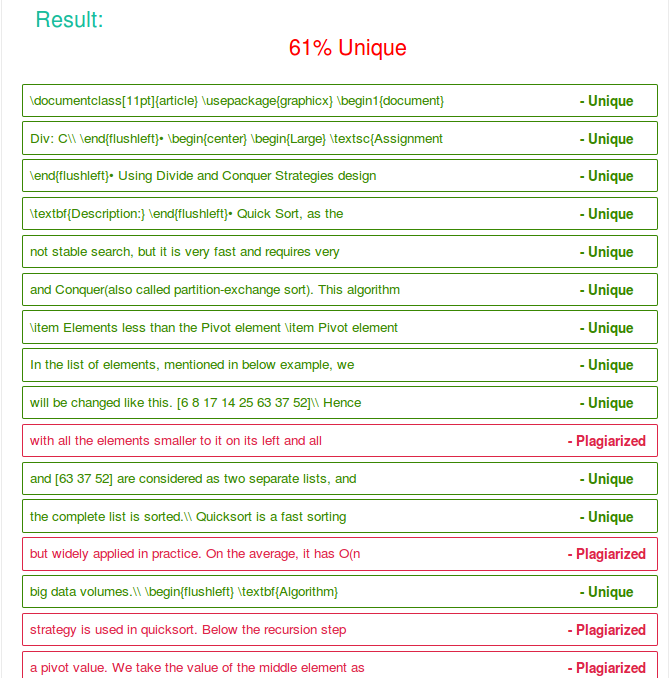
\includegraphics[width=\textwidth]{obst_plag}
\end{document}
 

 
